\documentclass[onecolumn, a4paper, 10pt]{article}

%%% Packages
\usepackage{graphicx}
\usepackage{balance}
\usepackage{tikz}
\usepackage{standalone}
\usepackage{colortbl}
\usepackage{subcaption}
\usepackage{amssymb}
\usepackage{amsmath}
\usepackage{amsfonts}
\usepackage{multirow,bigdelim}
\usepackage[pdftex, letterpaper, lmargin = 1.15in, rmargin = 1.15in]{geometry}

%%% TikZ libraries
\usetikzlibrary{backgrounds, positioning, decorations.pathreplacing, calc, fit}
\usetikzlibrary{shapes}

%%% Macros
\newcommand{\tbr}{{\color{red}\textbf{[TO BE REVISED]}}}
\newcommand{\tbd}{{\color{red}\textbf{[TO BE DONE]}}}

%\setlength{\parskip}{1em}

\begin{document}

% Title
\title{
  Spanner: Google's Globally-Distributed Database \newline
  Seminar Report
}

\author{
  Daniel Kocher \\
  Department of Computer Sciences \\
  University of Salzburg \\                                                    
  Daniel.Kocher@stud.sbg.ac.at
}

\maketitle

\section{Introduction}
\label{sec:introduction}

In the original paper~\cite{Corbett:2012}, Google introduced a
globally-distributed database referred to as \emph{Spanner}. This system is based
upon Paxos~\cite{Lamport:1998} state machines running on machines spread across
multiple datacenters across the world. This global replication guarantees high
availability and also implies some desirable locality properties which benefit
the performance.

Google already has two other highly scalable distributed databases, i.e.
Bigtable~\cite{Chang:2008} and Megastore~\cite{Baker:2011}. Hence, there must be
a reason, why they did not just use one of these but implemented another
distributed database. According to Google, it is difficult for applications/users
to deal with complex and evolving schemas in Bigtable. Moreover, Bigtable only
guarantees to be eventually-consistent. In contrast, Spanner provides much
stronger consistency guarantees. On the other hand, Megastore suffers from poor
write throughput even though many applications use it.

Therefore, Google decided to introduce another distributed, highly available and
scalable database system which evolved from a key-value store somehow similar to
the one used in Bigtable (but we will see that this is only partially correct).
A core feature provided by Spanner are so-called \emph{externally-consistent}
distributed general-purpose transactions. Of course, Spanner also provides an
SQL-like query language to enable applications/users to interact with Spanner in
a familiar way. The data is stored in schematized \emph{semi-relational} tables
and the data is versioned automatically. Google also implemented a garbage
collection to deal with old data. The replication can be dynamically configured
in order to control the locality of replicas. This is useful to control write
and read latency as well as availability. Another main contribution of Spanner
are high-performance \emph{globally-consistent} reads at a specific timestamp.
This and externally-consistent reads and writes enable Spanner to provide a
special type of transaction, so-called \emph{schema-change} transactions, which
provide atomic schema changes without blocking the whole database.

To provide all these features, Google designed a novel \emph{TrueTime} API which
exposes clock uncertainty and enables Spanner to assign commit timestamps to
transactions which reflect serialization order.

\section{Implementation}
\label{sec:implementation}

A Spanner deployment is referred to as a \emph{universe} which consists of
multiple zones. A universe has two global components: A \emph{universemaster}
which is a debugging console and shows the status of each zone. A
\emph{placement driver} which automatically moves data between zones due to
modified replication constraints or load balancing between zones.

Each zone is controlled by a \emph{zonemaster}. A zonemaster is responsible to
organize the data placement in a zone. The data is stored on so-called
\emph{spanservers} and the zonemaster assigns data to these spanservers. A zone
consists of multiple such spanservers which serve the data to clients. Spanner
somehow needs to enable the client to locate the spanservers which serve the data.
For this purpose, each zone contains multiple \emph{location proxies}.

According to Google, a zone can be seen as a Bigtable server deployment. The set
of zones also determines the locations across which the data can be replicated.
One can also think of a zone as geographically wide-spread locations, e.g.
continents. Using this kind of physical isolation, Spanner is resistent to events
which affect large areas, e.g. natural disasters or war. Hence, a well-configured
Spanner deployment is available almost all the time.
Figure~\ref{subfig:spanner-universe} illustrates the organization of a Spanner
universe.

\begin{figure}[ht]
  \centering
  \begin{subfigure}{0.45\textwidth}
    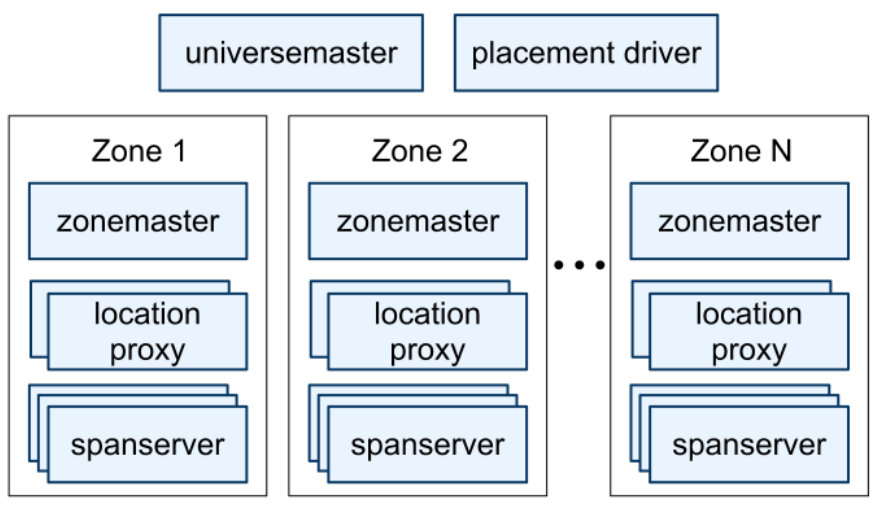
\includegraphics[width = \textwidth]{figs/spanner-server-organization.png}
    \caption{Spanner universe.~\cite{Corbett:2012}}
    \label{subfig:spanner-universe}
  \end{subfigure}
  \hfill
  \begin{subfigure}{0.45\textwidth}
    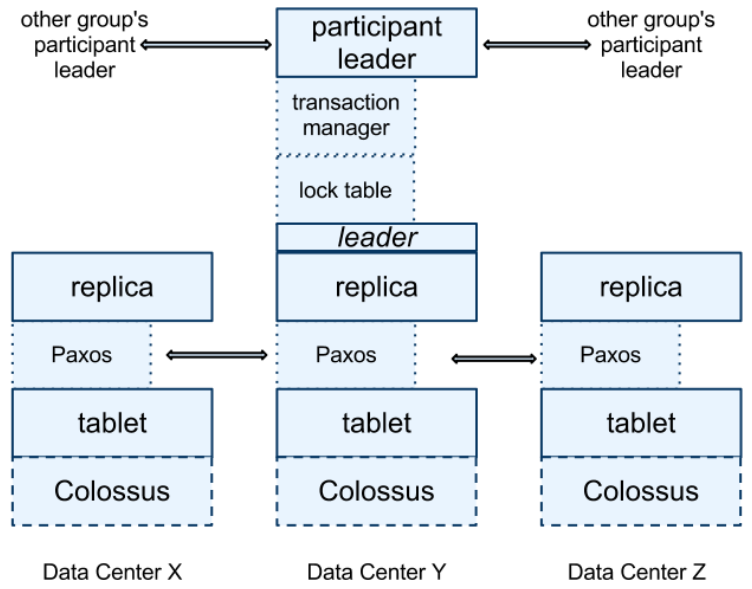
\includegraphics[width = \textwidth]{figs/spanserver-software-stack.png}
    \caption{Spanserver software stack.~\cite{Corbett:2012}}
    \label{subfig:spanserver-software-stack}
  \end{subfigure}
  \caption{Spanner hierarchy.}
  \label{fig:spanner-hierarchy}
\end{figure}

\subsection{Spanserver Software Stack \tbr}
\label{subsec:spanserver-software-stack}

Each spanserver again consists of multiple software layers (four at least). At
the bottom layer, every spanserver is responsible for between 100 and 1,000
\emph{tablets}. A tablet is bag of key-value mappings of the form
\begin{center}
  \texttt{(key:string, timestamp:int64)} $\rightarrow$ \texttt{value}
\end{center}
This is somehow similar to the tablet abstraction used in Bigtable. However,
Spanner \emph{automatically} assigns timestamps to data which makes Spanner a
\emph{multi-version} database. The state of a tablet is stored on a distributed
file system called \emph{Colossus}, the successor of the Google File
System~\cite{Ghemawat:2003}.

On top of each tablet, a Paxos state machine is implemented in order to support
consistent replication. One Paxos state machine is elect as leader. Leader leases
are assigned in a long-lived manner (default lease length is 10 seconds). A leader
implements three additional layers. A \emph{lock table} which stores the state
for two-phase locking and therefore implements the concurrency control. On top
of the lock table, a \emph{transaction manager} is implemented to coordinate
distributed transactions. In turn, this transaction manager is used to implement
a \emph{participant leader}. This leader is only utilized if a transaction
involves multiple Paxos groups (set of replicas). In this case, one of the
participant groups is chosen as coordinator and the leader of this group is
referred to as \emph{coordinator leader}.
Figure~\ref{subfig:spanserver-software-stack} shows the spanserver software stack.

\subsection{Directories}
\label{subsec:directories}

The next abstraction in the hierarchy is a bucketing abstraction. Google calls
this abstraction \emph{directory}. A directory is a set of contiguous keys.
All keys in a directory share a common prefix.

A directory is the unit of data placement/movement, hence only whole directories
are moved between Paxos groups, even across zones. Figure~\ref{subfig:directories}
illustrates this principle. Directory 2 is moved from Paxos group 1 to Paxos group
2 and, at the same time, from zone 2 to zone 3. Google shortly mentions that this
is an over-simplified view because a directory is split into multiple
\emph{fragments} if it grows too large. However, Google does not provide any
additional details.

All the data within a directory has the same replication configuration. As will
be described later, the concept of directories enables Google to improve the
performance of Spanner by placing directories which are frequently accessed
together in the same Paxos group. The fact that in general multiple directories
are placed in the same Paxos group is another difference between the key-value
mapping of Spanner and the one used in Bigtable. A Spanner tablet may contain
multiple contiguous ranges of keys (= directories) as opposed to a Bigtable tablet
which may only contain one contiguous range of keys.
Figure~\ref{fig:comparison-tablets} shows an example comparison of the two tablet
types.

\begin{figure}[ht]
  \centering
  \begin{subfigure}{0.45\textwidth}
    \centering
    \begin{tabular}{|l||ll}
      \hline
      {\bfseries Key} & {\bfseries Value} \tabularnewline
      \hline\hline
      12341 & \ldots & \rdelim\}{3}{5mm}[Directory 1234] \tabularnewline
      12342 & \ldots \tabularnewline
      12343 & \ldots \tabularnewline
      \hline
      67891 & \ldots & \rdelim\}{4}{3mm}[Directory 6789] \tabularnewline
      67892 & \ldots \tabularnewline
      67893 & \ldots \tabularnewline
      67894 & \ldots \tabularnewline
      \hline
    \end{tabular}
    \caption{Spanner tablet}
    \label{subfig:spanner-tablet}
  \end{subfigure}
  \qquad
  \begin{subfigure}{0.45\textwidth}
    \centering
    \begin{tabular}{|l||l}
      \hline
      {\bfseries Key} & {\bfseries Value} \tabularnewline
      \hline\hline
      12341 & \ldots \tabularnewline
      12342 & \ldots \tabularnewline
      12343 & \ldots \tabularnewline
      12344 & \ldots \tabularnewline
      12345 & \ldots \tabularnewline
      12346 & \ldots \tabularnewline
      12347 & \ldots \tabularnewline
      \hline
    \end{tabular}
    \caption{Bigtable tablet}
    \label{subfig:bigtable-tablet}
  \end{subfigure}
  \caption{Comparison of Spanner's and Bigtable's tablet}
  \label{fig:comparison-tablets}
\end{figure}

This partitioning of the row space is critical for the performance of Spanner
because it allows Google to physically \emph{co-locate} data that is frequently
accessed together. Therefore, directories are the smallest unit for which an
application/user can specify geographic-replication properties. An application
can control replication in two dimensions, namely the number and types of
replicas, and the geographic placement of replicas.

\begin{figure}[ht]
  \centering
  \begin{subfigure}{0.45\textwidth}
    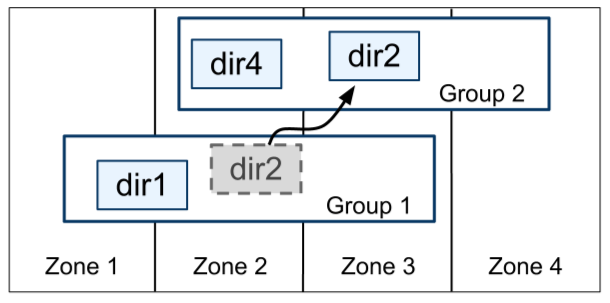
\includegraphics[width = \textwidth]{figs/directories}
    \caption{Directories (unit of data movement).~\cite{Corbett:2012}}
    \label{subfig:directories}
  \end{subfigure}
  \qquad
  \begin{subfigure}{0.45\textwidth}
    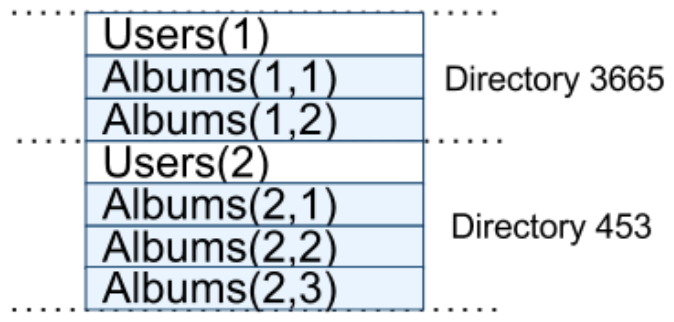
\includegraphics[width = \textwidth]{figs/interleaving-example.png}
    \caption{Two interleaved tables.~\cite{Corbett:2012}}
    \label{subfig:interleaved-tables}
  \end{subfigure}
  \caption{Directories and interleaved tables.}
  \label{fig:directories-and-tables}
\end{figure}

\subsection{Data Model}
\label{subsec:data-model}

There exists another layer on top of the directory-bucketed key-value mappings.
This layer is probably the most intuitive one for people who are used to common
database systems. The data model allows applications to create databases in a
universe each of which may contain any number of schematized
\emph{semi-relational} tables. A table has rows, columns and, as a third
dimension, versioned values. Spanner's tables are semi-relational because rows
must have names, i.e. every table must have an ordered set of one or more
primary-key columns. This is useful for applications because the locality of
data can be controlled by choosing keys accurately.

Therefore, Spanner requires the application/user to partition databases into
one or more hierarchies of tables. Based on this hierarchical information, Spanner
builds the directories. A directory contains hierarchically ordered rows from
all tables of a hierarchy which belong to the same key of the topmost table of
the hierarchy. Figure~\ref{subfig:interleaved-tables} shows an example of this
concept. In this example, the \texttt{Users} table is the topmost table of the
hierarchy and the \texttt{Albums} table is one level below. As we can see, all
rows of \texttt{Albums} connected to user \texttt{1} are located in the same
directory (\texttt{3365}). This directory has a common prefix, i.e. \texttt{1},
from the \texttt{Users} table. The same principle can be seen for key \texttt{2}
of the \texttt{Users} table. This interleaving of tables exploits locality
relationships of multiple tables and therefore is significant for Spanner's
performance.

\section{TrueTime}
\label{sec:truetime}

This section describes the key enabler of Spanner, i.e. the novel \emph{TrueTime}
API. Essentially, this API enables Google to assign timestamps to distributed
transactions which reflect serialization order.

TrueTime represents time as a $TTinterval$. A $TTinterval$ is an interval with a
bounded time uncertainty and has two endpoints, i.e. $earliest$ and $latest$,
which are of type $TTstamp$ (which is a timestamp in the context of Spanner).
Table~\ref{tbl:truetime-api} summarizes the three methods provided by the TrueTime
API. However, the most important method is $TT.now()$ which returns a $TTinterval$
which is guaranteed to contain the absolute time of the invocation of $TT.now()$,
i.e. $TT.now().earliest \leq t_{abs}(e) \leq TT.now().latest$, where $e$ denotes
the event of invoking $TT.now()$. More precisely, the absolute time of invocation
of $TT.now()$ is exactly in the middle this $TTinterval$. The interval itself
spans over $2\cdot\epsilon$, where $\epsilon$ denotes the instantaneous error
bound. $\epsilon$ is derived from applied worst-case local clock drift (assumed
to be $200\mu$s/sec). This instantaneous error bound is adjusted over time for
every single machine.

TrueTime uses GPS and atomic clocks as time references. Google chose these two
types of time references because the failure modes of them are uncorrelated. A
datacenter typically consists of multiple \emph{time master} machines. Most of
these are GPS receivers with dedicated antennas. All remaining time master
machines use an atomic clock as reference. Machines using an atomic clock as time
reference are referred to as \emph{Armageddon} masters. The references of all time
masters are compared against each other on a regular basis. To avoid incorrect
time references, time masters also cross-check their local clock drift against
the clock drift of the reference. If these differ too much, the time master evicts
itself.

Each machine has a \emph{timeslave daemon} installed which polls a variety of
time masters, mostly GPS masters but also some Armageddon masters. There is also
a mechanism to detect and reject liars which ensures that timeslave daemons only
synchronize to nonliars. 

\begin{table}[ht]
  \centering
  \begin{tabular}{|l||l|}
    \hline
    {\bfseries Method} & {\bfseries Returns} \tabularnewline
    \hline\hline
    $TT.now()$ & $TTinterval$: [$earliest$, $latest$] \tabularnewline
    \hline
    $TT.after(t)$ & true if $t$ has definitely passed \tabularnewline
    \hline
    $TT.before(t)$ & true if $t$ has definitely not arrived \tabularnewline
    \hline
  \end{tabular}
  \caption{Methods provided by the TrueTime API.}
  \label{tbl:truetime-api}
\end{table}

\section{Concurrency Control}
\label{sec:concurrency-control}

The TrueTime API allows Spanner to guarantee some correctness properties of the
implemented concurrency control. These enable some of the main features, i.e.
externally-consistent transactions, lock-free read-only transactions and so-called
\emph{snapshot reads}. Snapshot reads are non-blocking reads in the past at a
specific timestamp $t$. In this case, Spanner guarantees that snapshot reads will
see the effects of all transactions committed as of $t$.

Spanner provides different operations, as can be seen in
Table~\ref{tbl:reads-writes}. Read-only transactions have to be made explicit.
This requires the application/user to predeclare that the read-only transaction
does not include write operations. Moreover, read-only transaction have the
benefits of snapshot isolation because they are \emph{lock-free}. Standalone
writes are simply read-write transaction without any read operations. Non-snapshot
standalone reads are implemented as read-only transactions. Read-only transactions
and snapshot reads proceed on any \emph{sufficiently up-to-date} replica. For
snapshot reads, the application/user has two options. On the one hand, a precise
timestamp can be specified at which the read should be executed. On the other
hand, an upper bound can be specified and Spanner choses a timestamp that
satisfies this bound. 

\begin{table}
  \centering
  \begin{tabular}{|l||l|l|}
    \hline
    {\bfseries Operation} & {\bfseries Concurrency Control} &
    {\bfseries Replica required} \tabularnewline
    \hline\hline
    Read-Write transaction & Pessimistic & leader \tabularnewline
    \hline
    Read-Only transaction & Lock-free & leader; any
    \tabularnewline
    \hline
    Snapshot Read, client-provided timestamp & Lock-free & any \tabularnewline
    \hline
    Snapshot Read, client-provided bound & Lock-free & any \tabularnewline
    \hline
  \end{tabular}
  \caption{Reads and writes in Spanner.}
  \label{tbl:reads-writes}
\end{table}

\subsection{Paxos Leader Leases}
\label{subsec:paxos-leader-leases}

The Paxos implementation of Spanner is designed for long-lived leaderships. As
usual in Paxos implementations, a leader is elected by a quorum of lease votes.
If a machine receives such a quorum of lease votes, it gets a lease (10 seconds
by default). The lease vote of a replica is extended automatically on successful
writes.

Spanner enforces a \emph{disjointness invariant} such that for each Paxos group,
each Paxos leader's \emph{lease interval} is disjoint from every other leader's.
In order to guarantee this invariant, Spanner constrains abdication of leaders.
It defines a maximum timestamp used by a leader, denoted as $s_{max}$, which is
advanced by several transactions. A leader must not abdicate before
$TT.after\left(s_{max}\right)$ has passed.

\subsection{Read-Write Transactions}
\label{subsec:read-write-transactions}

Read-write transactions use two-phase locking and Spanner may only assign
timestamps in between the two phases. Spanner enforces another invariant, i.e. a
\emph{monotonicity invariant}, which makes use of the disjointness invariant.
This monotonicity invariant guarantees that within each Paxos group, Spanner
assigns timestamps to Paxos writes in monotonically increasing order. To guarantee
this across leaders, Spanner utilizes the disjointness invariant. This implies
that a leader must only assign timestamps within the interval of its leader
lease. $s_{max}$ is advanced to $s$ whenever a timestamp $s$ is assigned by a
leader.

To guarantee externally-consistent reads and writes, Spanner enforces an
\emph{external consistency invariant}. In essence, this invariant guarantees that
whenever the commit of a transaction $T_1$, denoted as $e_1^{commit}$, occurs
before the start of a transaction $T_2$, denoted as $e_2^{start}$, then the commit
timestamp of $T_1$, denoted as $s_1$, is guaranteed to be smaller than the
timestamp of $T_2$, denoted as $s_2$. More formally, the following must hold to
guarantee external consistency:
\begin{center}
$t_{abs}\left(e_1^{commit}\right) < t_{abs}\left(e_2^{start}\right) \Rightarrow s_1 < s_2$
\qquad\qquad $t_{abs}(e)$ \ldots absolute time of an event $e$
\end{center}

\noindent
Spanner obeys two rules in order to guarantee this invariant:
\begin{description}
  \item[Start] Coordinator leader for a write $T_i$ assigns a commit timestamp
    $s_i \geq TT.now().latest$, where $TT.now()$ is executed right after the
    arrival event of the commit request for $T_i$.
  \item[Commit Wait] Coordinator leader ensures that clients cannot see data
    committed by $T_i$ until $TT.after\left(s_i\right)$ is true. This ensures
    that the assigned timestamp $s_i$ is less than the absolute commit time of
    $T_i$.~\cite{Corbett:2012}
\end{description}

Figure~\ref{fig:read-write-transaction} illustrates the timeline of a distributed
read-write transaction. There are three participants groups involved, i.e. $P_2$,
$P_3$ and $P_{CL}$ (which is the coordinator leader). In the first step, all three
participants acquire their locks and execute $TT.now()$ right afterwards to obtain
timestamps independently. Every participant logs his timestamp through Paxos and
after this was done, sends its timestamp to the coordinator leader. The
coordinator leader then computes an overall timestamp for the transaction. This
timestamp must be greater than any timestamp the leader has assigned before,
greater or equal to all timestamps received from the participants and greater than
$TT.now().latest$ at the time the coordinator leader received the commit message.
Then, the computed timestamp is logged by the coordinator leader through Paxos
but no participants are notified until the commit wait rule is satisfied. After
commit wait is satisfied, the coordinator leader notifies all other participants
which are allowed to release their locks after receiving this notification.

\begin{figure}
  \centering
  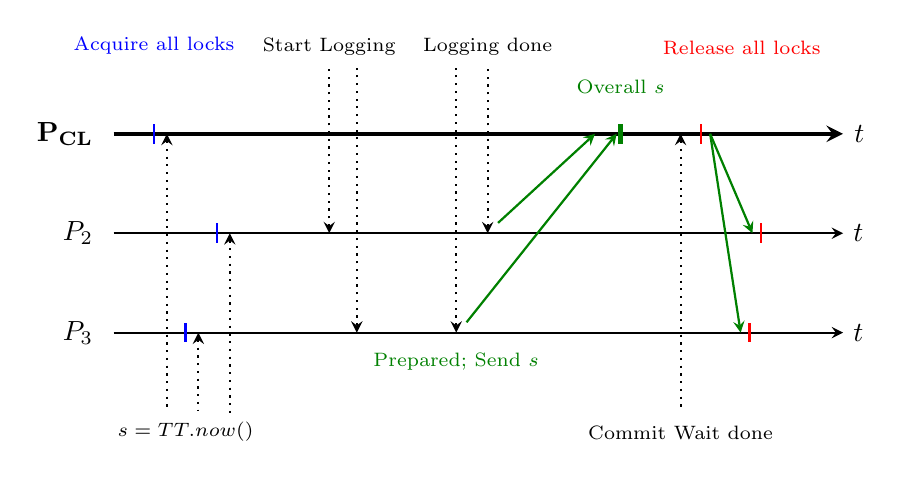
\begin{tikzpicture}[thick, scale = 0.5]
    \node (left-end-t1) at (0,2) {};
    \node[right = 9 of left-end-t1] (right-end-t1) {};
    \draw[ultra thick, ->, >=stealth] (left-end-t1.center) -- (right-end-t1.center)
      node[right] (right-end-t1-t) {$t$};
    \node[left = 0 of left-end-t1.west] (left-end-t1-t) {$\mathbf{P_{CL}}$};

    \node[below = 1 of left-end-t1] (left-end-t2) {};
    \node[right = 9 of left-end-t2] (right-end-t2) {};
    \draw[->, >=stealth] (left-end-t2.center) -- (right-end-t2.center)
      node[right] (right-end-t2-t) {$t$};
    \node[left = 0 of left-end-t2.west] (left-end-t2-t) {$P_2$};

    \node[below = 1 of left-end-t2] (left-end-t3) {};
    \node[right = 9 of left-end-t3] (right-end-t3) {};
    \draw[->, >=stealth] (left-end-t3.center) -- (right-end-t3.center)
      node[right] (right-end-t3-t) {$t$};
    \node[left = 0 of left-end-t3.west] (left-end-t3-t) {$P_3$};

    \node[right = 0.25 of left-end-t1] (acquire-locks-t1) {};
    \node[right = 1.05 of left-end-t2] (acquire-locks-t2) {};
    \node[right = 0.65 of left-end-t3] (acquire-locks-t3) {};
    \foreach \x in {1, 2, 3}{
      \draw[blue] (acquire-locks-t\x.center) -- ++(0, -0.25);
      \draw[blue] (acquire-locks-t\x.center) -- ++(0, 0.25);
    }

    \node[above = 0.75 of acquire-locks-t1]
      (acquire-locks-t) {\scriptsize\color{blue}Acquire all locks};
    
    \foreach \x in {1, 2, 3}{
      \node[right = -0.1 of acquire-locks-t\x] (compute-s-t\x) {};
    }
    \node[below = 1 of acquire-locks-t3.center]
      (compute-s-t) {\scriptsize $s=TT.now()$};
    \draw[<-, >=stealth, dotted] (compute-s-t1.center) -- ++(0, -7);
    \draw[<-, >=stealth, dotted] (compute-s-t2.center) -- ++(0, -4.6);
    \draw[<-, >=stealth, dotted] (compute-s-t3.center) -- ++(0, -2);
    
    \node[right = 1 of compute-s-t2] (start-log-t2) {};
    \node[right = 1.75 of compute-s-t3] (start-log-t3) {};
    \node[above = 2 of start-log-t2] (start-log-t)
      {\scriptsize Start Logging};
    \draw[<-, >=stealth, dotted] (start-log-t2.center) -- ++(0, 4.25);
    \draw[<-, >=stealth, dotted] (start-log-t3.center) -- ++(0, 6.75);
    
    \node[right = 1 of start-log-t3] (end-log-t3) {};
    \node[right = 1.75 of start-log-t2] (end-log-t2) {};
    \node[above = 2 of end-log-t2] (end-log-t)
      {\scriptsize Logging done};
    \draw[<-, >=stealth, dotted] (end-log-t2.center) -- ++(0, 4.25);
    \draw[<-, >=stealth, dotted] (end-log-t3.center) -- ++(0, 6.75);
    \node[right = 5.5 of compute-s-t1] (compute-s-global) {};
    \draw[<-, >=stealth, black!50!green] (compute-s-global) ++(-0.1, 0) --
      (end-log-t3.north east);
    \draw[<-, >=stealth, black!50!green] (compute-s-global) ++(-0.65, 0) --
      (end-log-t2.north east);
    \draw[black!50!green, ultra thick] (compute-s-global.center) -- ++(0, -0.25);
    \draw[black!50!green, ultra thick] (compute-s-global.center) -- ++(0, 0.25);

    \node[above = 0.25 of compute-s-global] (compute-s-global-t)
      {\scriptsize\color{black!50!green} Overall $s$};
    \node[below = 0 of end-log-t3] (prepared-t)
      {\scriptsize\color{black!50!green}Prepared; Send $s$};
    
    \node[right = 0.5 of compute-s-global] (commit-wait-done) {};
    \node[below = 3.45 of commit-wait-done] (commit-wait-done-t)
      {\scriptsize Commit Wait done};
    \draw[<-, >=stealth, dotted] (commit-wait-done.center) -- ++(0, -7);
    \node[right = 0 of commit-wait-done] (release-locks-t1) {};
    \draw[red] (release-locks-t1.center) -- ++(0, -0.25);
    \draw[red] (release-locks-t1.center) -- ++(0, 0.25);
    \node[above right = 0.75 and -0.75 of release-locks-t1]
      (release-locks-t1-t) {\scriptsize\color{red}Release all locks};
    
    \node[right = -0.15 of release-locks-t1] (notify-t1) {};
    \node[right = 3.1 of end-log-t2] (notify-t2) {};
    \node[right = 3.35 of end-log-t3] (notify-t3) {};
    \foreach \x in {2, 3}{
      \draw[->, >=stealth, black!50!green] (notify-t1.center) --
        (notify-t\x.center); 
    }
    
    \node[right = -0.15 of notify-t2] (release-locks-t2) {};
    \node[right = -0.15 of notify-t3] (release-locks-t3) {};
    \draw[red] (release-locks-t2.center) -- ++(0, -0.25);
    \draw[red] (release-locks-t2.center) -- ++(0, 0.25);
    \draw[red] (release-locks-t3.center) -- ++(0, -0.25);
    \draw[red] (release-locks-t3.center) -- ++(0, 0.25);
  \end{tikzpicture}
  \caption{Timeline of a read-write transaction.}
  \label{fig:read-write-transaction}
\end{figure}

This also explains why, according to Table~\ref{tbl:reads-writes}, Read-write
transactions only involve the \emph{leader} replicas. Only the leader replicas
of each participant communicate with the coordinator leader. Hence, no other
replicas are involved.

\subsection{Snapshot Reads}
\label{subsec:reads-at-timestamp}

In order to provide snapshot reads, we first need to define
\emph{sufficiently up-to-date}. Therefore Spanner tracks a \emph{safe time},
denoted as $t_{safe}$, at each replica. $t_{safe}$ is defined as the maximum
timestamp at which the corresponding replica is up-to-date. Hence, a replica
satisfies reads at every timestamp $t$ if $t \leq t_{safe}$ holds. Spanner can
then perform a snapshot read at any replica that is sufficiently up-to-date. As
a consequence, snapshot reads have the same performance benefits as provided by
snapshot isolation since they are totally lock-free. 

The safe time is determined by the safe time of a Paxos state machine, denoted
as $t_{safe}^{Paxos}$, and the safe time of the transaction manager, i.e.
$t_{safe}^{TM}$. The overall safe time of a replica then is the minimum of
these two.

$t_{safe}^{Paxos}$ is simply assigned the time of the highest-applied Paxos write
because if the Paxos level is reached in the spanserver software stack, then the
corresponding transaction has already been committed. $t_{safe}^{TM}$ is $\infty$
if there exists a distributed transaction which is in between the two phases of
the two-phase commit because in this case the system does not know if this
transaction will commit.

\subsection{Read-Only Transactions}
\label{subsec:read-only-transactions}

Read-only transactions are also lock-free and execute in two phases. In the first
phase, a timestamp $s_{read}$ is assigned. In the second phase, the read-only
transaction is executed as a snapshot read at $s_{read}$. Spanner assigns
the oldest timestamp which preserves external consistency to $s_{read}$.

In general, read-only transactions involve group leaders but they may also involve
any other sufficiently up-to-date replica in the process. Group leaders are
involved in the negotiation phase. In this phase, all involved Paxos groups
negotiate in order to determine $s_{read}$. To accomplish this, Spanner requires
every read-only transaction to define a \emph{scope} expression which summarizes
all keys that will be read by the respective transaction.

If all values of the scope can be served by a single Paxos group, the client
issues the read-only transaction to the corresponding group leader. The group
leader then assigns the timestamp of the last committed write to $s_{read}$ and
executes the transaction.

If serving the values of the scope involves multiple Paxos groups, Spanner avoids
a negotiation round (which would be a viable option). Instead, Spanner simply
assigns $TT.now().latest$ to $s_{read}$, even though this may have to wait for
$t_{safe}$ to advance.

In both cases, the snapshot read at $s_{read}$ can execute on any sufficiently
up-to-date replica. The leader replicas are only involved in the negotiation
phase.

\subsection{Schema-Change Transactions}
\label{subsec:schema-change-transactions}

Schema-change transactions are variants of standard transactions which change
schemas atomically without blocking any other transactions.

There are two phases involved. In the first phase, the \emph{prepare} phase,
Spanner explicitly assigns a future timestamp to the schema-change transaction.
In the subsequent phase, reads and writes synchronize with any registered
schema-change timestamp at time $t$. Of course, this affects only reads and
writes which implicitly depend on the modified schema. Any read/write transaction
may proceed if its timestamp preceeds $t$. If its timestamp is after $t$, the
corresponding read/write has to block behind the schema-change transaction. This
is essentially enabled by the TrueTime API because without TrueTime, it would
not be guaranteed that the timestamp of the schema-change transaction is in the
future on every single machine.

\section{Performance}
\label{sec:performance}

\begin{table}[ht]
  \centering
  { \footnotesize
    \begin{tabular}{|l||l|l|l||l|l|l|}
      \hline
      & \multicolumn{3}{c||}{{\bfseries Latency in [ms] (less is better)}} &
      \multicolumn{3}{c|}{{\bfseries Throughput in [Kops/sec] (more is better)}}
      \tabularnewline
      \cline{2-7}
      {\bfseries Replicas} & {\bfseries Write} & {\bfseries RO Transaction} &
      {\bfseries Snapshot Read} & {\bfseries Write} &
      {\bfseries RO Transaction} & {\bfseries Snapshot Read} \tabularnewline
      \hline\hline
      1D & $9.4\pm0.6$ & - & - & $4.0\pm0.3$ & - & - \tabularnewline
      \hline
      1 & $14.4\pm1.0$ & $1.4\pm0.1$ & $1.3\pm0.1$ & $4.1\pm0.05$ &
      $10.9\pm0.4$ & $13.5\pm0.1$ \tabularnewline
      \hline
      3 & $13.9\pm0.6$ & $1.3\pm0.1$ & $1.2\pm0.1$ & $2.2\pm0.5$ &
      $13.8\pm3.2$ & $38.5\pm0.3$ \tabularnewline
      \hline
      5 & $14.4\pm0.4$ & $1.4\pm0.05$ & $1.3\pm0.04$ & $2.8\pm0.3$ &
      $25.3\pm5.2$ & $50.0\pm1.1$ \tabularnewline
      \hline
    \end{tabular}
  }
  \caption{Performance of operations. Mean and standard deviation over 10
    runs.~\cite{Corbett:2012}
  }
  \label{tbl:performance-of-operations}
\end{table}

This section summarizes the core results of the evaluation of Spanner, i.e. the
latency and throughput performance as well as some results concerning availability
and the TrueTime API.

Table~\ref{tbl:performance-of-operations} summarizes the latency and throughput
performance of Spanner. 1D means one replica with Commit Wait disabled. Hence,
only write transactions are evaluated because Commit Wait is not involved in any
other type of transaction. As we can see, the latency of all transaction types is
almost stable for an increasing number of replicas whereas the standard deviation
decreases. The throughput of read-only transactions increases with the number of
replicas because the number of spanservers increases. In the experiments, the
number of replicas and the number of spanservers were equal. The throughput of write
transactions also benefits from this fact. However, the number of write operations
to perform increases linearly with the number of replicas. This explains why the
throughput of write transactions does not increase with the number of replicas.
Snapshot reads benefit the most from the Spanner architecture. The throughput of
snapshot reads increases almost linearly with the number of replicas. 

The availability of Spanner is only affected if zones containing multiple leaders
are shut down without notifying the leaders upfront. In this case, it takes Spanner
about 10s to recover. If the leaders are notified to abdicate before their zone
is shut down, the availability is almost unaffected. The same is true if a zone
without a leader is shut down.

Google also provided empirical results about TrueTime. All assumptions Google
made while designing Spanner would be broken if the local clock drift of a machine
exceeds $200\mu$s/sec. But Google found that clock issues are extremely infrequent
relative to more serious hardware problems, e.g. bad CPUs. Moreover, Google
provided empirical results on the values of $\epsilon$. Typically, $\epsilon$ is
never larger than 10ms. It decreases as the network infrastructure is improved
and increases if time masters go offline.

\section{Future Work}
\label{sec:future-work}

Google plans to implement optimistic parallel reads but it turned out that
implementing it is non-trivial. They also want to support direct configuration
changes of the Paxos state machines and to reduce $\epsilon$ to be $\leq 1ms$ in
order to improve the performance if data is sharded between nearby datacenters.

Moreover, the node-local performance could be improved for complex queries. By
now, node-local data structures are designed for key-value accesses and these data
structures could be improved by algorithms and data structure from database
literature.

To improve the performance even further, Google plans to move processes between
datacenters if the data on which they operate is moved. This would have high
impact because the performance of the processes is close to optimal if the data
is as local as possible. However, moving processes between datacenters raises
even more complex problems.

\section{Discussion}
\label{sec:discussion}

The system introduced by Google is definitely impressive because they were able
to establish a notion of global wall clock time (that's how they call it in their
presentation). Global wall clock time enables them to guarantee serialization order
for globally-distributed transactions. To the best of the author's knowledge, Spanner
was the first system to provide much stronger consistency and time semantics while
data is sharded and replicated at global scale. Google also proved all
'\emph{Relational databases are dead}' people wrong even though systems like
Bigtable helped creating the NoSQL trend. Reading about a system like Spanner is
definitely more than a vital sign of relational database systems. From a
developer's point of view, this is interesting because Spanner provides
the more intuitive schematized view of tables. In contrast to NoSQL database
systems, Spanner can be used as replacement for other relational database
systems, e.g. MySQL, directly. Spanner is also highly flexible to schema changes
because it supports atomic schema change transactions.

However, I believe that rebuilding a Spanner-like system is difficult for
small- to mid-sized companies because there is a lot of hardware involved, for
example all the GPS and atomic clocks. Unless this hardware infrastructure is
available it is hard to reimplement the TrueTime API. Nonetheless,
companies which need a globally-distributed database with all the guarantees
Spanner provides are likely to be almost as big as Google. Hence, such companies
would also have the resources to build a Spanner-like system. An Open-Source
reimplementation would only be possible if every datacenter would provide GPS
and Armageddon time masters on their own.

A component that may influence the performance of Spanner is the distributed
file system, i.e. Colossus, the successor of the Google File System. The internet 
does not provide reliable information about the implementation or the performance
of Colossus. It is unknown how much impact this distributed file system has on the
performance of Spanner. Thus, it is hard to say if a reimplementation of Spanner
would be able to compete with Spanner's performance if a different distributed
file system is used.

Of course, a distributed database system may also be built upon other concepts,
e.g. the Network Time Protocol (NTP). But this would result in poor performance
compared to Spanner because the error interval would be much larger then the one
used by Spanner, i.e. $2\cdot\epsilon$. And besides providing distributed
general-purpose transactions, it is the performance of Spanner that impressives
the most. A system using NTP would never be able to achieve this performance
while guaranteeing serialization order of transactions. Spanner can synchronize
multiple systems without any communication between these systems. NTP-based
systems would have to communicate with each other. For systems far apart such a
NTP-based solution would never be able to compete with Spanner.

Spanner is robust to GPS blackouts because of the usage of atomic clocks, even
though the performance of Spanner may suffer due to high values of $\epsilon$.
Would be interesting to see how a GPS blackout would affect Spanner's performance.

It would also be interesting to know how failures of the two singletons per
universe, i.e. universemaster and placement driver, would affect Spanner. Since
the universemaster is just a debugging console, most probably a failure in this
component will not affect Spanner at all. This would probably be a totally
different story if the placement driver does not operate correctly. First of all,
there would be no load balancing between zones. Hence, zones could run out of
space if the placement driver is down long enough. Furthermore, updated
replication constraints, would not be propagated since the placement driver is
responsible to move the data if the replication constraints are modified.
Therefore I do not understand why there is no redundancy in placement driver.

In terms of applications, applications which read a lot but write rarely or little
data would benefit the most from a system like Spanner. If an application uses
lots of replicas which are spread across the globe and writes large amounts of data
regularly, Spanner may not provide the performance presented in the original
publication. However, Spanner may still outperform all other distributed database
systems while providing much stronger consistency guarantees.

%\clearpage
\bibliographystyle{abbrv}
\bibliography{paper}

\end{document}
